\chapter{Weighted Interval Scheduling\normalfont{\emoji{man-lifting-weights}}}

Questo algoritmo cerca di ottenere un insieme di intervalli non sovrapposti
(\textit{overlapping}) che è il più grande possibile. Per la versione senza pesi
($weight = 1$) esiste uno specifico algoritmo greedy che è in grado di trovare la
soluzione ottima, tuttavia nella versione pesata ($weight \neq 1$) sarà
necessario utilizzare la programmazione dinamica.

\section{Costi}

%% TODO: migliorare sta tabella
\begin{center}
    \begin{tabular}{|c|c|}
        \textbf{Funzione}    & \textbf{Costo}                \\
        \verb|Compute-Opt|   & esponenziale (forse $O(2^n)$) \\
        \verb|M-Compute-Opt| & $O(n)$                        \\
        \verb|Find-Solution| & $O(n)$
    \end{tabular}
\end{center}

\section{Notazioni}

Per discutere il problema dell'Interval Scheduling, utilizzeremo la seguente
notazione:

\begin{itemize}
    \item $n$: un intero che rappresenta l'indice dell'intervallo (job)
    \item $s_i$: tempo di inizio dell'intervallo $i$
    \item $f_i$: tempo di fine dell'intervallo $i$
    \item $v_i$: peso dell'intervallo $i$
    \item $p(j)$: ritorna l'indice più grande $i$, con $i < j$, del primo
          intervallo compatibile con l'intervallo $j$, considerando il fatto che gli
          intervalli sono ordinati in ordine non decrescente in base a $f_i$
    \item $\mathcal{O}_j$: rappresenta la soluzione ottima al problema calcolato
          sull'insieme $\{1, \ldots, j\}$
    \item $OPT(j)$: rappresenta il valore della soluzione ottima $\mathcal{O}_j$
\end{itemize}

\begin{figure}[H]
    \centering
    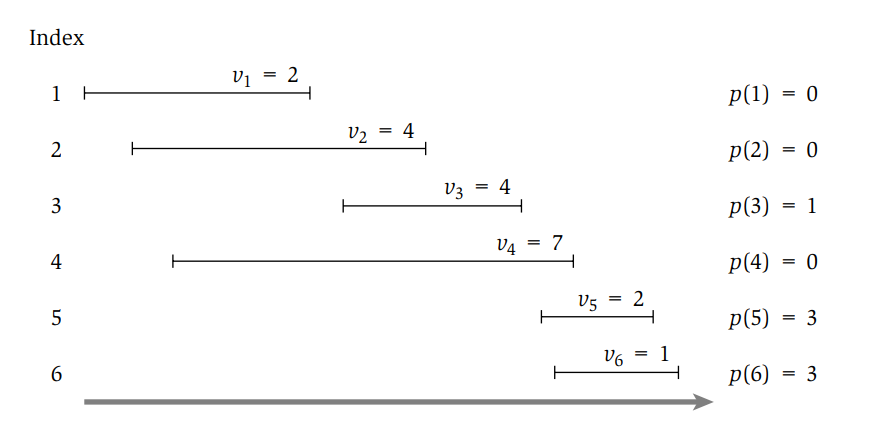
\includegraphics[width=12cm, keepaspectratio]{capitoli/imgs/weighted_problem.png}
    \caption{Istanza di un problema.}
\end{figure}

\section{Goal \normalfont{\emoji{soccer-ball}}}

L'obiettivo del nostro problema attuale è quello di trovare un sottoinsieme $S
    \subseteq \{1, \ldots, n\}$ di intervalli mutualmente compatibili che vanno a
massimizzare la somma dei pesi degli intervalli selezionati $\sum_{i \in S}
    v_i$.

\section{Funzionamento}

Come prima cosa definiamo il metodo per calcolare $OPT(j)$. Il problema è
una \textit{scelta binaria} che va a decidere se l'intervallo di indice $j$
verrà incluso nella soluzione oppure no basandosi sul valore ritornato dalla
seguente formula:

\begin{equation}
    \label{eqn:weight-opt}
    OPT(j) = max(v_j + OPT(p(j)), \ \ OPT(j-1))
\end{equation}
\ \\
Questo può essere anche visto come una disequazione:

\begin{equation}
    \label{eqn:weight-opt-dis}
    v_j + OPT(p(j)) \geq OPT(j-1)
\end{equation}
\ \\
che se vera, includerà $j$ nella soluzione ottimale.

\pagebreak

Scrivendo tutto sotto forma di algoritmo ricorsivo avremmo che:

\begin{lstlisting}[language=Javascript]
    function Compute-Opt(j){
        if (j == 0)
            return 0
        else
            return max(vj+Compute-Opt(p(j)), Compute-Opt(j − 1))
    }
\end{lstlisting}

Costruendo l'albero della ricorsione dell'algoritmo si nota che la complessità
temporale è esponenziale \emoji{astonished} !

\begin{figure}[H]
    \centering
    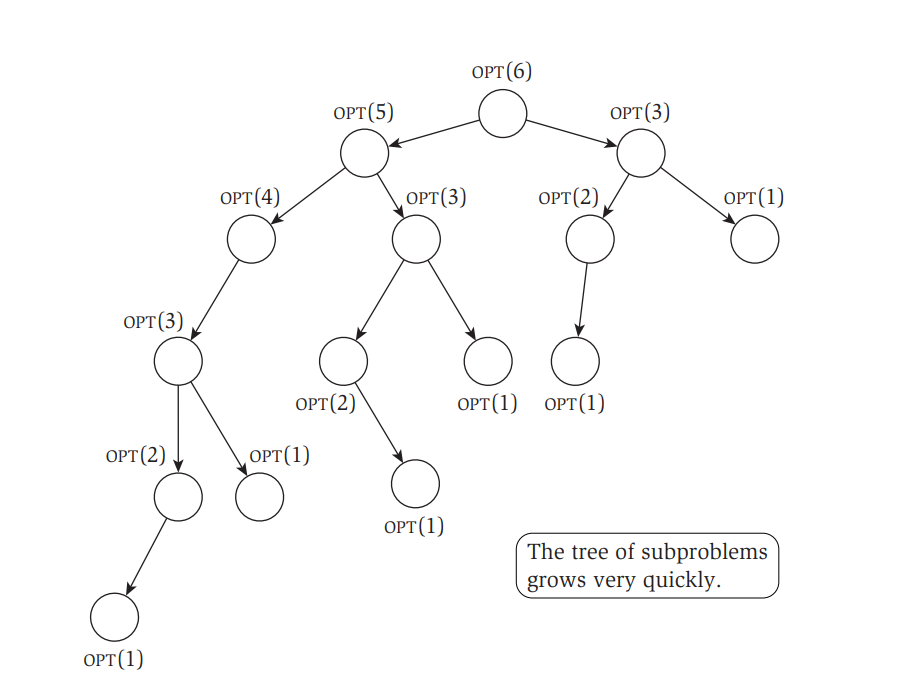
\includegraphics[width=12cm, keepaspectratio]{capitoli/imgs/opt_albero.png}
    \caption{Sviluppo dell'albero di ricorsione per la risoluzione di un problema.}
\end{figure}

\pagebreak

Una soluzione è quella di utilizzare la tecnica della \textbf{Memoization} che evita
di ricalcolare $OPT$ per gli indici già calcolati precedentemente, rendendo così
il costo temporale uguale ad $O(n)$ \emoji{man-in-motorized-wheelchair}.

\begin{lstlisting}[language=Javascript]
function M-Compute-Opt(j){
    if (j == 0)
        return 0
    else if (M[j] is not empty)
        return M[j]
    else
        let M[j] = max(vj+M-Compute-Opt(p(j)), M-Compute-Opt(j-1))
        return M[j]
}
\end{lstlisting}

Oltre al valore della soluzione ottimale probabilmente vorremmo sapere anche
quali sono gli intervalli che la compongono, e intuitivamente verrebbe da creare
un array aggiuntivo in cui verranno aggiunti gli indici degli intervalli
ottenuti con \verb|M-Compute-Opt|. Tuttavia questo aggiungerebbe una complessità
temporale di $O(n)$ peggiorando notevolmente le prestazioni. Un'alternativa è
quella di recuperare le soluzioni dai valori salvati nell'array \verb|M| dopo che la
soluzione ottimale è stata calcolata. Per farlo possiamo sfruttare la formula
vista in precedenza $v_j + OPT(p(j)) \geq OPT(j-1)$, che ci permette di
rintracciare gli intervalli della soluzione ottima.

\begin{lstlisting}[language=Javascript]
    function Find-Solution(j) {
        if (j == 0)
            Output nothing
        else if (vj + M[p(j)] >= M[j-1])
            Output j together with the result 
            of Find-Solution(p(j))
        else
            Output the result of Find-Solution(j-1)
    }
\end{lstlisting}